%!TEX root = ../presa.tex
\documentclass[12pt,pdf,hyperref={unicode}, dvipsnames]{beamer}
\usepackage[english,russian]{babel}
% \usepackage[T2A,T1]{fontenc}
\usepackage[utf8]{inputenc}
\usepackage{tikz}
\usepackage[unicode]{hyperref}
\usepackage{pgfplots,standalone}
% \usepackage{lmodern}
\pgfplotsset{compat=newest} 
\usetikzlibrary{%
    decorations.pathreplacing,%
    decorations.pathmorphing,%
    patterns,%
    angles,%
    quotes,%
    calc, %
    3d, %
    backgrounds, %
    positioning%
}

% Стиль презентации
\usetheme{Warsaw}

% \setbeamercolor{frametitle right}{fg=white,bg=Brown!85}
% \setbeamercolor{frametitle}{fg=white,bg=Brown!85}
\setbeamercolor{frametitle right}{fg=white,bg=black!85!blue}
\setbeamercolor{frametitle}{fg=white,bg=black!85!blue}

\setbeamertemplate{frametitle}[default][colsep=-4bp,rounded=false,shadow=false]
% \setbeamertemplate{frametitle}
% {
%     \nointerlineskip
%     \begin{beamercolorbox}[sep=0.3cm,ht=1.8em,wd=\paperwidth]{frametitle}
%         \vbox{}\vskip-2ex%
%         \strut\insertframetitle\strut
%         \vskip-0.8ex%
%     \end{beamercolorbox}
% }
\setbeamercolor{section in head/foot}{fg=white, bg=black!75}
\setbeamertemplate{frametitle}{%
    \nointerlineskip%
    \begin{beamercolorbox}[wd=\paperwidth,ht=2.5ex,dp=1.6ex]{frametitle}
        \hspace*{1ex}\insertframetitle%
    \end{beamercolorbox}%
}
\setbeamertemplate{headline}{}
\setbeamertemplate{footline}{}
\let\Tiny=\tiny % решает проблему со шрифтами в TexLive
% \setbeamertemplate
% 	{footline}{
% 		\color{black!40!white}
% 		\quad\hfill
% 		\insertframenumber/\inserttotalframenumber
% 		\hfill\vspace{1em}\quad
% 	} 

\setbeamertemplate{navigation symbols}{}

\beamersetrightmargin{0.5cm} 
\beamersetleftmargin{0.5cm}

\setbeamertemplate{enumerate item}{
	\usebeamercolor[bg]{item projected}
    \tikz[baseline = -4pt]{\draw[fill=black!95] (0,0) circle (3pt);}%
	% \raisebox{1pt}{\colorbox{bg}{\color{fg}\footnotesize\bf\insertenumlabel}}%
}
\setbeamertemplate{enumerate subitem}{ 
    \usebeamercolor[bg]{item projected}
    \tikz[baseline = -4pt]{\draw[fill=black!95] (0,0) circle (2.5pt);}%
    % \raisebox{1pt}{\colorbox{bg}{\color{fg}\footnotesize\bf\insertenumlabel.\insertsubenumlabel}}%
}
\setbeamercolor{item projected}{bg=black,fg=white}

% \setbeamertemplate{itemize item}{%
% 	\usebeamercolor[bg]{item projected}%
% 	\raisebox{1pt}{{\color{bg}\footnotesize$\bf\square$}}%
% }
% \setbeamercolor{item projected}{bg=black,fg=white}
\setbeamercolor{title}{bg=black!85!blue,fg=white}

\newcommand\frametitless[1]{\subsection{#1}\frametitle{#1}}

\usepackage{booktabs, setspace}
\usepackage{esdiff,esint}
\newcommand{\tabitem}{~~\llap{\textbullet}~~}
\setbeamertemplate{caption}{\raggedright\insertcaption\par}


\usepackage[font=footnotesize,justification=centering]{caption}
\captionsetup[figure]{labelformat=empty}%
% \setbeamertemplate{caption}[default]
\usefonttheme{professionalfonts}
\defbeamertemplate*{background canvas}{mydefault}
    {%
      \ifbeamercolorempty[bg]{background canvas}{}{\color{bg}\vrule width\paperwidth height\paperheight}% copied beamer default here
    }

    \defbeamertemplate*{background canvas}{bg}
    {%
      \color{black}\vrule width\paperwidth height\paperheight% added bg color
    }

    \BeforeBeginEnvironment{frame}{%
      \setbeamertemplate{background canvas}[mydefault]%
    }

    \makeatletter 
    \define@key{beamerframe}{bg}[true]{%
      \setbeamertemplate{background canvas}[bg]%
    }
    \makeatother

\newcommand{\sq}[1]{\tikz{\draw[draw=#1,fill=#1] (0,0) rectangle (0.7em,0.7em);}}
\usepackage{xcolor}
\definecolor{ochre}{HTML}{e2431e} % #e2431e 0
\definecolor{lightorange}{HTML}{e7711b} % #e7711b 1
\definecolor{lightyellow}{HTML}{f1ca3a} % #f1ca3a 2
\definecolor{lightgreen}{HTML}{6f9654} % #6f9654 3
\definecolor{osci}{HTML}{82FF27}%#82FF27
\definecolor{sky}{HTML}{1c91c0} % #1c91c0 4
\definecolor{violet}{HTML}{43459d} % #43459d 5
\title[]{Исследование диэлектриков с помощью квазиоптических резонаторов Фабри-Перро}
\institute{Радиофизический факультет ННГУ, 430 группа}
\date{Нижний Новгород, 2018}
\usepackage[makeroom]{cancel}
\usepackage{tabu}
\begin{document}  
% \end{document}
%%%%%%%%%%%%%%%%%%%%%%%%%%%%%%%%%%%%%%%%%%%%%%%%%%%%%%%%%%%%%
\begin{frame}[plain]
	\centering
	\vspace{1.2cm}
	\begin{beamercolorbox}[sep=8pt,center]{title}
		\bf\usebeamerfont{title}\inserttitle
	\end{beamercolorbox}
	\vspace{0.5cm}
	\normalsize \textbf{Работу выполнили:}\\
	\large
	\underline{Платонова М.В.}, %
	{Сарафанов Ф.Г.}, %
	{Новиков А.Г.}
	% {Рогов М.А.}, #wasted
	% {Геликонова В.Г.}, % #wasted
	\\ 
	\vspace{0.5cm}
	\normalsize{\textbf{Научный руководитель:}\\}
	% \large{Яковлев А.И.}
	% \large{Антипов О.Л.}
	% \large{Щапин Д.С.}
	% \large{Мареев Е.А.}
	% \large{Пестов Е.Е.}
	\large{Паршин В.В.}
	\vfill
	\small{Нижний Новгород -- 2018}
\end{frame}
%%%%%%%%%%%%%%%%%%%%%%%%%%%%%%%%%%%%%%%%%%%%%%%%%%%%%%%%%%%%%
% \begin{frame}[t]s
% 	\frametitle{Содержание}
% 	% \fontsize{6pt}{7.2}\selectfont
% 	\setbeamerfont{subsection in toc}{size=\tiny}
% 	\setbeamerfont{section in toc}{size=\tiny}
% 	\tableofcontents
% \end{frame}
%%%%%%%%%%%%%%%%%%%%%%%%%%%%%%%%%%%%%%%%%%%%%%%%%%%%%%%%%%%%%

\section{Введение}
\subsection{Цели работы}
\begin{frame}[t]
	\frametitle{Цели работы}
	% \textbf{Цели}\\
	\vfill
	\begin{spacing}{1}
		\begin{enumerate}
			\item Исследовать распространение гауссовых пучков в открытом резонаторе Фабри-Перро
			\item Рассмотреть применение открытых резонаторов для исследования свойств диэлектриков 
			\item Измерить показатель преломления диэлектрической пластины (в качестве пластины -- алмазное окно гиратрона) и тангенс угла диэлектрических потерь
% CVD-Diamond , t=1.8mm
		\end{enumerate}
	\end{spacing}
	\vfill
\end{frame}

\subsection{Распределение поля в гауссовом пучке}
\begin{frame}[c]%[bg]
	\frametitle{Распределение поля в гауссовом пучке}
	\vspace{-1em}
	\begin{columns}[t]
		\begin{column}{0.49\textwidth}%\centering
			\begin{figure}[h]
				% \hspace{-2em}
				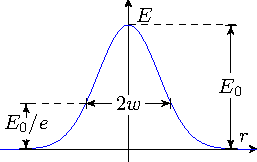
\includegraphics[width=0.86\linewidth]{ris/E}
				\caption{Поперечное распределение}
				% \vspace{1em}
			\end{figure}
		\end{column}
		\begin{column}{0.49\textwidth}%\centering
			\begin{figure}[h]
				% \hspace{-2em}
				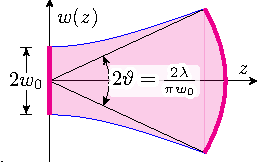
\includegraphics[width=0.86\linewidth]{ris/w}
				\caption{Продольное распределение }
			\end{figure}

		\end{column}
	\end{columns}
	\begin{columns}[b]
		\begin{column}{0.49\textwidth}%\centering
			$$
				E(r)=E_0\exp\left[-\frac{r^2}{w^2}\right]
			$$
		\end{column}
		\begin{column}{0.49\textwidth}%\centering
			$$
				w^2(z)=w_0^2\left[1+\left(\frac{\lambda z}{\pi w_0^2}\right)^2\right]
			$$
		\end{column}
	\end{columns}			
	\begin{columns}[b]
		\begin{column}{0.49\textwidth}%\centering
			$$
				R(z)=z\left[1+\left(\frac{\pi w_0^2}{\lambda z}\right)^2\right]
			$$
		\end{column}
		\begin{column}{0.49\textwidth}%\centering
			$$
				\Phi(z)=\arctg\left(\frac{\lambda z}{\pi w_0^2}\right)
			$$
		\end{column}
	\end{columns}
\end{frame}

\subsection{Открытый резонатор Фабри-Перро}
\begin{frame}[c]%[bg]
	\frametitle{Открытый резонатор Фабри-Перро}
	\vspace{-2em}
	% \vspace{-0.5em}
	% У открытых резонаторов $L \gg \lambda$
	\begin{columns}[b]
	\begin{column}{0.49\textwidth}%\centering
	\begin{figure}[H]
		% \hspace{-9pt}
		\centering
		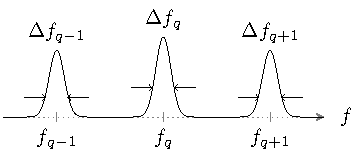
\includegraphics[scale=1]{ris/fq}
		\caption{Резонансные частоты}
		\label{fig:chem}
	\end{figure}
	\end{column}
	\begin{column}{0.49\textwidth}%\centering
	\begin{figure}[H]
		% \hspace{-9pt}
		\centering
		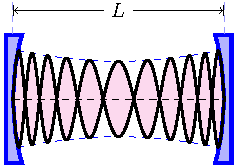
\includegraphics[scale=1]{ris/fabri}
		\caption{Узлы стоячей волны
		 % в резонаторе ($R_1=R_2\equiv R,\,\, d=L$)
		 }
		\label{fig:chem}
	\end{figure}	
	\end{column}
	\end{columns}
	\vspace{-0.5em}
	\begin{equation*}
		L_\text{рез}=
			 \underbrace{\frac{\lambda q}{2}}_{\substack{\text{q -- кол-во}\\\text{полуволн}}}+
			\underbrace{\frac{\lambda}{2\pi}\arccos\left(1-\frac{L}{R}\right)}_{\substack{\text{увеличение расстояния}\\\text{между нулями}\\\text{в гауссовом пучке}}}
			\underbrace{-{\frac{\lambda^2}{8\pi^2 R}}}_{\substack{\text{учет}\\\text{несферичности}\\\text{волнового фронта}}}
		% \pi q=\frac{2\pi L}{\lambda}-2\arctg\left(\frac{\lambda d}{\pi \omega_0^2}\right)
	\end{equation*}
	\begin{equation*}
		f_\text{рез}=\frac{c}{2L}\cdot\left[
			q+\frac{1}{\pi}\arccos\left(1-\frac{L}{R}\right)
		\right]
	\end{equation*}
\end{frame}


\subsection{Диаграмма устойчивости}
\begin{frame}[c]%[bg]
	\frametitle{Диаграмма устойчивости резонатора}
	\vspace{-1.07em}
	% \vspace{-0.5em}
	\begin{figure}[H]
		% \hspace{-9pt}
		\centering
		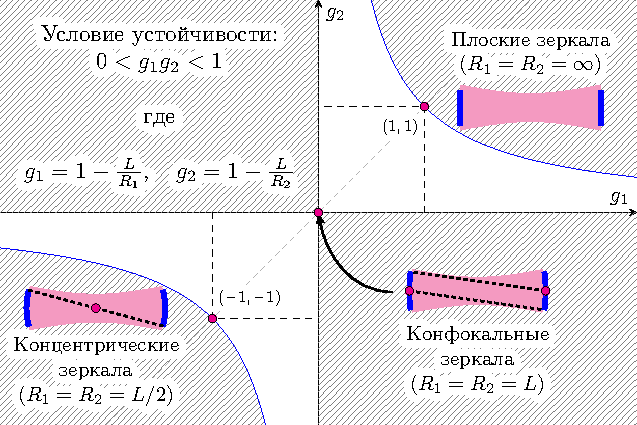
\includegraphics[scale=1.1]{ris/diagram}
		\label{fig:chem}
	\end{figure}	
\end{frame}

\subsection{Потери в резонаторе}
\begin{frame}[c]%[bg]
	\frametitle{Потери в резонаторе}
	\vspace{-1em}
	\begin{columns}[t]
		\begin{column}{0.44\textwidth}%\centering
			\vspace{-2em}
			\begin{figure}[h]
				% \hspace{-2em}
				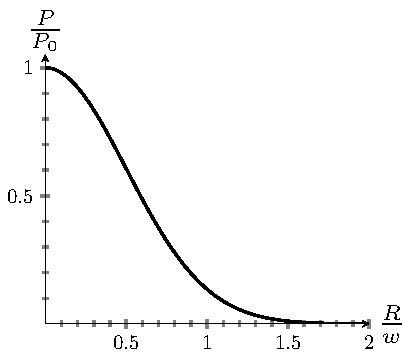
\includegraphics[width=1\linewidth]{ris/p}
				\caption{Дифракционные потери}
				\vspace{-0.8em}
			\end{figure}
		\begin{equation*}
			P_\text{диф}=P_0\exp\left(-\frac{2R^2}{w^2}\right)
		\end{equation*}	
		% При $R/w\sim 2.4$, $P/P_0\sim 10^{-5}$
			% \vspace{0.7em}
			% $$
			% \vartheta=\frac{\lambda}{\pi w_0}
			% $$
		\end{column}
		\begin{column}{0.55\textwidth}%\centering

\begin{tabu} to \textwidth { | X[1.5,c] | X[c] | X[c] | X[c] |}
 \hline
 $P_\text{диф}/P_0$ & $10^{-1}$ & $10^{-3}$ & $10^{-5}$ \\
 \hline
 $R/w$  & 1.07 & 1.86 & 2.4 \\
\hline
\end{tabu}

			\begin{equation*}
				P_\Sigma=(P_\text{связи}+P_\text{зерк})+P_\text{зап}+\xcancel{P_\text{диф}}
			\end{equation*}
			\begin{enumerate}
				\item Дифракционные потери можно сделать пренебрежимо малыми
				\item Собственные потери резонатара можно найти в ненагруженном режиме 
			\end{enumerate}

		\end{column}
	\end{columns}
\end{frame}

\section{Эксперимент}
\subsection{Cхема экспериментальной установки}
\begin{frame}[b]%[bg]
	\frametitle{Cхема экспериментальной установки}
	\vspace{-0.7em}
	% \vspace{-0.5em}

	\begin{figure}[H]
		\centering
		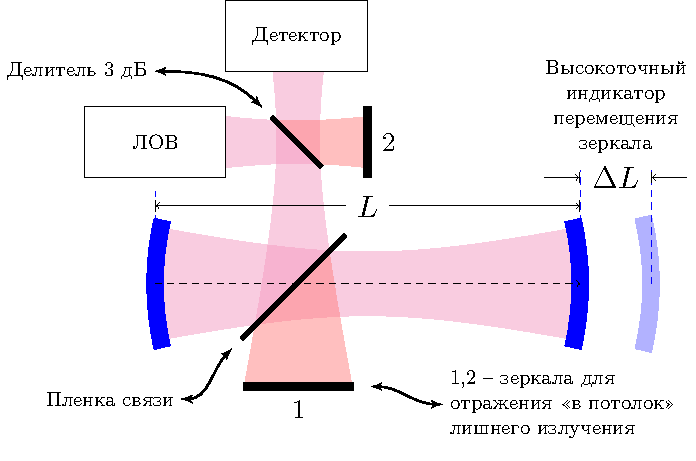
\includegraphics[]{ris/chem_exp}
		% \caption{Еще не нарисована. Будет: 1) пленка связи (+описание ее преимуществ устно) 2) ЛОВ, ФАПЧ, устройство измерения dL и прочие устройства}
		\label{fig:chem}
	\end{figure}	
\end{frame}

\subsection{Поиск резонансной частоты}
\begin{frame}[c]%[bg]
	\frametitle{Поиск резонансной частоты}
	% \vspace{-1em}
	\vspace{-0.5em}
	\begin{columns}[t]
		\begin{column}{0.49\textwidth}%\centering
			\vspace{-1em}
			\begin{figure}[H]
				\centering
				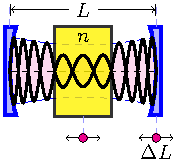
\includegraphics[width=0.8\linewidth]{ris/dl}
				% \caption{}
				\label{fig:chem}
			\end{figure}
			\vspace{-2.5em}
			\begin{figure}[H]
				\centering
				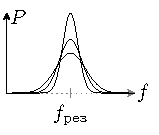
\includegraphics[width=0.8\linewidth]{ris/fres}
				% \caption{}
				\label{fig:chem}
			\end{figure}
		\end{column}
		\begin{column}{0.49\textwidth}%\centering
			\begin{enumerate}
				\item Приблизительно отцентровали диэлектрик на оси резонатора
				\item Одновременно перестраивая пределы свипа по частоте источника и изменяя длину резонатора, нашли резонансную частоту, при которой смещение диэлектрика не вызывает смещения резонансного пика
			\end{enumerate}
		\end{column}
	\end{columns}
		
\end{frame}

\subsection{Расчет показателя преломления}
\begin{frame}[t]%[bg]
	\frametitle{Расчет показателя преломления}
	\vspace{-1em}
	\vspace{-0.5em}
	\begin{gather*}
	\left\{
		\begin{aligned}
			t\cdot n=& \frac{q_d \lambda_1}{2}\\
			t\cdot n=& \frac{(q_d+1) \lambda_2}{2}
		\end{aligned}
	\right.\quad\Rightarrow\quad
	q_d=\frac{\lambda_2}{\lambda_2-\lambda_1}
	\end{gather*}
	\begin{gather*}
		L_\text{рез1}=
			 \frac{\lambda (q+q_d/n)}{2}+
			\frac{\lambda}{2\pi}\arccos\left(1-\frac{L_\text{рез1}}{R}\right)\\
		L_\text{рез2}=
			 \frac{\lambda (q+q_d)}{2}+
			\frac{\lambda}{2\pi}\arccos\left(1-\frac{L_\text{рез2}}{R}\right)
	\end{gather*}
	\begin{equation*}
	\hspace{-0.5em}
				n=q_d\left[
			q_d-\frac{2\Delta L}{\lambda}+\frac1\pi\cos^{-1}\left(1-\frac{L_\text{рез1}}{R}\right)-\frac1\pi\cos^{-1}\left(1-\frac{L_\text{рез2}}{R}\right)
		\right]^{-1}
	\end{equation*}
	% Запишем условие когда оптическая толщина пластины составляет целое число 
	% полуволн: tn = mo/2.    Для следующей полуволны: tn=(m+1)1/2.
	% Отсюда находим  m = 1/(1-o). 
	% (Заметим, что  m  целое число и оно может быть определено как округлённое целое от выражения  2tn/, если известны заранее с достаточной  точностью величины показателя преломления и толщина образца.)  
	% Представив  t как m/2n, длина резонатора может быть записана как:
	% 	L = q/2 + m/2n + (/2) arccos (1-L/R)
	% где: L – расстояние между зеркалами; q – количество полуволн в свободном пространстве резонатора; R – радиус кривизны зеркал.
	% Более удобно измерять не длину резонатора, а её изменение (Δ), после изъятия диэлектрика и восстановления резонанса с прежним количеством полуволн (q+m).  	Для этого случая запишем:
	% 	L1 = q/2 + m/2n + (/2)arccos[1-L1/R]
	% 	Lo = q/2 + m/2   + (/2)arccos[1-Lo/R]
	% 	Отсюда находим  n:
	% n = m{m-2L/+[arccos(1-Lo/R)-arccos(1-L1/R)]/}-1   где: L=Lo-L1. 
	% Для резонатора длиной  L ~ 300 мм и толщине диэлектрика  t~10 мм, относительная точность расчёта показателя преломления по этим упрощенным формулам ~ 10-3.

	% \begin{columns}[t]
	% 	\begin{column}{0.49\textwidth}%\centering
	% 		\vspace{-1em}
	% 		\begin{figure}[H]
	% 			\centering
	% 			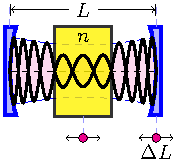
\includegraphics[width=0.8\linewidth]{ris/dl}
	% 			% \caption{}
	% 			\label{fig:chem}
	% 		\end{figure}
	% 		\vspace{-2.5em}
	% 		\begin{figure}[H]
	% 			\centering
	% 			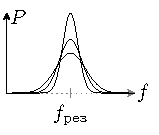
\includegraphics[width=0.8\linewidth]{ris/fres}
	% 			% \caption{}
	% 			\label{fig:chem}
	% 		\end{figure}
	% 	\end{column}
	% 	\begin{column}{0.49\textwidth}%\centering
	% 		\begin{enumerate}
	% 			\item Приблизительно отцентровали диэлектрик на оси резонатора
	% 			\item Одновременно перестраивая пределы свипа по частоте источника и изменяя длину резонатора, нашли резонансную частоту, при которой смещение диэлектрика не вызывает смещения резонансного пика
	% 		\end{enumerate}
	% 	\end{column}
	% \end{columns}
		
\end{frame}

\subsection{Измерение угла потерь}
\begin{frame}[c]%[bg]
	\frametitle{Измерение угла потерь}
	% \vspace{-1em}
	\vspace{-0.5em}
	\begin{columns}[c]
		\begin{column}{0.49\textwidth}%\centering
			\vspace{-0.7em}
			\begin{figure}[H]
				\centering
				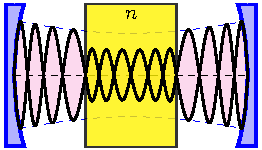
\includegraphics[width=0.6\linewidth]{ris/f-}
				\caption{Измерение $\Delta f_-$}
				\label{fig:chem}
			\end{figure}
			\vspace{-2.5em}
			\begin{figure}[H]
				\centering
				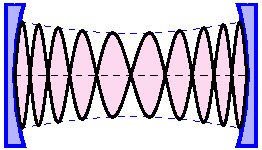
\includegraphics[width=0.6\linewidth]{ris/f0}
				% \caption{}
				\caption{Измерение $\Delta f_0$}
				\label{fig:chem}
			\end{figure}
			\vspace{-2.5em}
			\begin{figure}[H]
				\centering
				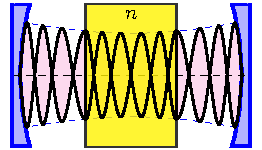
\includegraphics[width=0.6\linewidth]{ris/f+}
				\caption{Измерение $\Delta f_+$}
				\label{fig:chem}
			\end{figure}
		\end{column}
		\begin{column}{0.49\textwidth}%\centering
			Упрощённый расчет $\tan\delta$:
			\begin{gather*}
				\tan\delta=\frac{L\cdot(\Delta f_--\Delta f_0)}{tf}\\
				\tan\delta=\frac{L\cdot(\Delta f_+-\Delta f_0)}{tfn^2}\\
				\tan\delta=\frac{L\cdot(\Delta f_+-\Delta f_-)}{tf(n^2-1)}
			\end{gather*}
			Тройное измерение дает относительную точность $\sim$ 10\%
			% \begin{equation*}
				% \Delta[\tan\delta]\sim 10^{-1} \div 10^{-5}
			% \end{equation*}
		\end{column}
	\end{columns}
		
\end{frame}

% % %%%%%%%%%%%%%%%%%%%%%%%%%%%%%%%%%%%%%%%%%%%%%%%%%%%%%%%%%%%%%
\section{Заключение}
\subsection{Выводы}
\begin{frame}
	\frametitle{Выводы}
	\begin{enumerate}
			\item Рассмотрен гауссов пучок и его распространение в открытом резонаторе Фабри-Перро
			\item Резонансным методом определен показатель преломления алмазного окна $n=2.38$ и тангенс угла диэлектрических потерь $\tan\delta=9.7\cdot10^{-6}$
			\item Найдена резонансная частота окна $f_\text{рез}=139853$ МГц
			\item Рассчитано, насколько нужно изменить толщину окна $t$, чтобы оно стало резонансным на частоте $f=140$ ГГц: $\Delta t=-1.7$ мкм 
			% (пилить не надо -- окно укладывается в границы допуска по частоте)
	\end{enumerate}
\end{frame}
% %%%%%%%%%%%%%%%%%%%%%%%%%%%%%%%%%%%%%%%%%%%%%%%%%%%%%%%%%%
\subsection{Спасибо за внимание}
\begin{frame}[plain]
	\vspace{4cm}
	\begin{center}
		\Huge
		Спасибо за внимание!
	\end{center}
	\vspace{2.5cm}
	\begin{center}
		\color{black!30!white}
		Презентация подготовлена в издательской \\
		системе LaTeX с использованием пакетов \\
		PGF/TikZ и Beamer
	\end{center}
\end{frame}

\subsection{Приложение}
\begin{frame}[plain]
	\begin{gather*}
		I=I_0\cdot\exp\left[\frac{-2r^2}{w^2}\right]
		\\% \qquad
		P_\text{диф}=\int\limits_{r>R}I(r)\cdot\mathrm{d}S=[dS=2\pi r \mathrm{d}r]=
		\int\limits_{R}^{\infty} I_0\cdot\exp\left[\frac{-2r^2}{w^2}\right] 2\pi r \mathrm{d}r=\\=
		%
		\pi I_0\int\limits_{R^2}^{\infty}\exp\left[\frac{-2r^2}{w^2}\right] \mathrm{d}\left[r^2\right]=
		%
		\left[x=\left[\frac{-2r^2}{w^2}\right]\right]
		=\\=
		\frac{-\pi I_0 w^2}{2}\int\limits_{-2R^2/w^2}^{-\infty} e^x \,\mathrm{d}x=\\=
		\frac{\pi I_0 w^2}{2}\exp\left(-\frac{2R^2}{w^2}\right)=P_0\exp\left(-\frac{2R^2}{w^2}\right)
	\end{gather*}
\end{frame}

\begin{frame}[plain]
	\begin{figure}[tb]
		\centering
		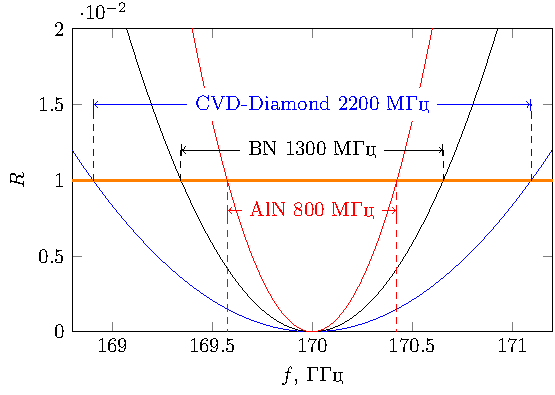
\includegraphics[]{ris/Rf}
		\caption{Допуск по частоте для разных материалов при допустимом отражении 0.01}
		\label{fig:figure1}
	\end{figure}
\end{frame}
\end{document}